\documentclass[11pt]{article}

\usepackage[T1]{fontenc}
\usepackage{geometry}
\usepackage{amsmath, amssymb, amsthm}
\usepackage[scr]{rsfso}
\usepackage[%
    hidealllines=true,%
    innerbottommargin=15,%
    nobreak=true,%
]{mdframed}
\usepackage{bm}
\usepackage{xcolor}
\usepackage{graphicx}
\usepackage{fancyhdr}
\usepackage{hyperref}
\usepackage{epstopdf}

\geometry{a4paper, margin=1in, headheight=14pt}

\pagestyle{fancy}
\fancyhf{}
\renewcommand\headrulewidth{0.4pt}
\fancyhead[L]{\scshape MA3102: Algebra I}
\fancyhead[R]{\scshape \leftmark}
\rfoot{\footnotesize\it Updated on \today}
\cfoot{\thepage}

\newcommand{\C}{\mathbb{C}}
\newcommand{\R}{\mathbb{R}}
\newcommand{\Q}{\mathbb{Q}}
\newcommand{\Z}{\mathbb{Z}}
\newcommand{\N}{\mathbb{N}}

\renewcommand{\vec}[1]{\boldsymbol{#1}}
\newcommand{\vv}{\vec{v}}
\newcommand{\vw}{\vec{w}}
\newcommand{\vx}{\vec{x}}
\newcommand{\vy}{\vec{y}}
\newcommand{\ve}{\vec{e}}
\newcommand{\va}{\vec{a}}
\newcommand{\vb}{\vec{b}}

\newcommand{\norm}[1]{\Vert #1 \Vert}
\newcommand{\ip}[2]{\langle #1, #2 \rangle}

\newmdtheoremenv[%
    backgroundcolor=blue!10!white,%
]{theorem}{Theorem}[section]
\newmdtheoremenv[%
    backgroundcolor=violet!10!white,%
]{corollary}{Corollary}[theorem]
\newmdtheoremenv[%
    backgroundcolor=teal!10!white,%
]{lemma}[theorem]{Lemma}

\theoremstyle{definition}
\newmdtheoremenv[%
    backgroundcolor=green!10!white,%
]{definition}{Definition}[section]
\newmdtheoremenv[%
    backgroundcolor=red!10!white,%
]{exercise}{Exercise}[section]

\theoremstyle{remark}
\newtheorem*{remark}{Remark}
\newtheorem*{example}{Example}
\newtheorem*{solution}{Solution}

\surroundwithmdframed[%
    linecolor=black!20!white,%
    hidealllines=false,%
    innertopmargin=5,%
    innerbottommargin=10,%
    skipabove=0,%
    skipbelow=0,%
]{example}

\numberwithin{equation}{section}

\title{
    \Large\textsc{MA3102} \\
    \Huge \textbf{Algebra I} \\
    \vspace{5pt}
    \Large{Autumn 2021}
}
\author{
    \large Satvik Saha
    \\\textsc{\small 19MS154}
}
\date{\normalsize
    \textit{Indian Institute of Science Education and Research, Kolkata, \\
    Mohanpur, West Bengal, 741246, India.} \\
}

\begin{document}
    \maketitle

    \tableofcontents

    \section{Symmetries}
    \subsection{Symmetries of plane figures}
    A symmetry of a plane figure can be thought of as a rigid motion which
    \emph{preserves its structure}, i.e.\ sends it to itself.

    For example, consider an equilateral triangle; there is the identity symmetry
    (which does nothing), two rotations by $2\pi / 3$ and $2\pi / 3$, and three
    reflections. This gives us a total of $6$ symmetries. Coincidentally, the plane
    symmetries of an equilateral triangle are precisely the set of $3! = 6$
    permutations of its vertices.

    \begin{center}
        \includegraphics[width=0.6\textwidth]{./triangle_square.eps}
    \end{center}

    The same cannot be said of a square; there are $4! = 24$ of its vertices, but
    only $8$ of them are rigid motions. Here, we see $4$ rotations and $4$
    reflections.

    In general, a regular $n$-gon has $2n$ plane symmetries, of which $n$ are
    rotations and $n$ are reflections. This can be seen by noting that a symmetry of
    an $n$-gon is completely determined by its action on an edge; once the final
    positions of the first two vertices is determined, the rest are forced. There are
    $n$ positions for the first vertex, which leaves only $2$ positions for the
    second vertex. One of these choices results in a rotation (since it preserves the
    cyclicity of the vertices) and the other a reflection (since it reverses the
    cyclicity of the vertices).

    Note that these symmetries can be \emph{composed}, i.e.\ applied in succession.
    For example, a rotation by $2\pi / n$ can be applied repeatedly to obtain every
    possible rotational symmetry. Similarly, we can perform rotations and reflections
    in succession, and we always end up with another symmetry. This composition is
    associative, there is an identity symmetry, and each symmetry has an inverse.
    The collection of such symmetries forms a \emph{group}.

    The group of plane symmetries of a regular $n$-gon is called the \emph{dihedral
    group}, denoted as $D_{2n}$.

    \subsection{Symmetries of the Euclidean plane}
    Consider the class of isometries of the plane, i.e.\ all bijections $f\colon \R^2
    \to \R^2$ such that $\norm{f(\vv) - f(\vw)} = \norm{\vv - \vw}$. These constitute
    symmetries of the Euclidean plane $\R^2$. The three basic forms of such
    symmetries are rotations, reflections, and translations; it can be shown that
    every symmetry of $\R^2$ is a combination of at most three reflections.  Another
    representation for each symmetry is \[
        f(\vv) = A\vv + \vv_0,
    \] where $A \in O_2(\R)$ is an orthogonal matrix, accounting for the rotational
    and reflectional part of the transformation.

    To show this, set $\vv_0 = f(\vec{0})$ and define $g = f - \vv_0$. Thus,
    $g(\vec{0}) = \vec{0}$, and $g$ is also an isometry.
    
    Not that for all $\vv, \vw \in \R^2$, we can write
    \begin{align*}
        \norm{g(\vv) - g(\vw)}^2 &= \norm{g(\vv)}^2 + \norm{g(\vw)}^2 -
        2\ip{g(\vv)}{g(\vw)}, \\
        \norm{\vv - \vw}^2 &= \norm{\vv}^2 + \norm{\vw}^2 -
        2\ip{\vv}{\vw}.
    \end{align*}
    On the other hand, $\norm{g(\vv) - g(\vw)}^2 = \norm{\vv - \vw}^2$, and
    $\norm{g(\vv)}^2 = \norm{\vv}^2$, $\norm{g(\vw)}^2 = \norm{\vw}^2$. This gives
    $\ip{g(\vv)}{g(\vw)} = \ip{\vv}{\vw}$, i.e.\ $g$ preserves the inner product.

    We claim that $g(\alpha\vv) = \alpha g(\vv)$ for all $\alpha \in \R$, $\vv
    \in \R^2$. Note that $\norm{g(\alpha\vv)} = \norm{\alpha\vv} = \norm{\alpha g(\vv)}$.
    Now,
    \begin{align*}
        \norm{g(\alpha\vv) - \alpha g(\vv)}^2 &= \norm{g(\alpha\vv)}^2 + \norm{\alpha
        g(\vv)}^2 - 2\ip{g(\alpha\vv)}{\alpha g(\vv)} \\
        &= \alpha^2v^2 + \alpha^2v^2 - 2\alpha\ip{\alpha\vv}{\vv} \\
        &= 2\alpha^2v^2 - 2\alpha^2v^2 \\
        &= 0.
    \end{align*}    
    This proves that $g(\alpha\vv) = \alpha g(\vv)$.

    Next, we claim that $g(\vv + \vw) = g(\vv) + g(\vw)$ for all $\vv, \vw \in
    \R^2$. Write
    \begin{align*}
        \norm{g(\vv + \vw) - g(\vv) - g(\vw)}^2 &= \norm{g(\vv + \vw) - g(\vv)}^2 +
        \norm{g(\vw)}^2 - 2\ip{g(\vv + \vw) - g(\vv)}{g(\vw)} \\
        &= \norm{\vv + \vw - \vv}^2 + \norm{\vw}^2 - 2\ip{\vv + \vw}{\vw} +
        2\ip{\vv}{\vw} \\
        &= w^2 + w^2 - 2\ip{\vv}{\vw} - 2w^2 + 2\ip{\vv}{\vw} \\
        &= 0.
    \end{align*}
    This proves that $g(\vv + \vw) = g(\vv) + g(\vw)$. Thus, $g$ is a linear map.

    Now let $g(\ve_1) = \va$ and $g(\ve_2) = \vb$. Clearly, $\norm{\va} = \norm{\vb}
    = 1$. For arbitrary $\vv\in \R^2$, we immediately get $g(\vv) = v_x\va + v_y\vb$,
    so by arranging $\va$ and $\vb$ as the columns of a $2\times 2$ matrix $A$, we
    have $g(\vv) = A\vv$. We clearly have $A^\top A = \mathbb{I}_2$ from $\va^\top\va
    = \vb^\top\vb = 1$, and $\ip{\va}{\vb} = \ip{\ve_1}{\ve_2} = 0$. Thus, $A \in
    O_2(\R)$. Substituting this back into $f$, we have \[
        f(\vv) = A\vv + \vv_0
    \] as desired.

    It can be further shown (algebraically) that every member of $O_2(\R)$ is of the
    form \[
        \begin{bmatrix}
            \cos\theta & \mp\sin\theta \\ \sin\theta & \pm \cos\theta
        \end{bmatrix}.
    \] 


    \subsection{Symmetries of the Petersen graph}
    Consider a graph $G(V, E)$. A symmetry of $G$ is a bijection $f\colon V \to V$
    on the set of vertices, which preserves the edges. In other words, it preserves
    the adjacency function. Thus, it can be shown that the degree of each vertex will
    be preserved by a symmetry.

    The following graph is called the Petersen graph, with 10 vertices and 15 edges.

    \begin{center}
        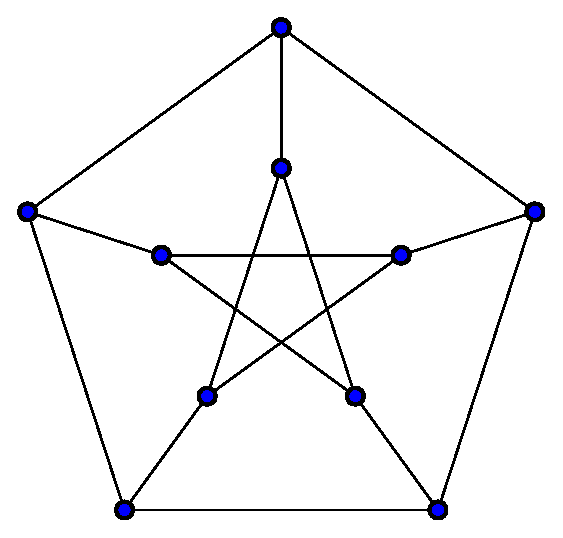
\includegraphics[width=0.5\textwidth]{./petersen.eps}
    \end{center}

    We can show that this graph has $120$ symmetries. This can be done by looking at
    all $2$ element subsets of $\{1, 2, 3, 4, 5\}$, of which there are $10$. Place
    these subsets as the vertices of a new graph, and connect two such sets with an
    edge if they \emph{are disjoint}. The resulting graph can be shown to be
    identical to the Petersen graph. It is immediately clear that any permutation of
    the set $\{1, 2, 3, 4, 5\}$ produces a relabelling of the vertices, which
    nevertheless preserves the Petersen graph. This gives us at least $5! = 120$
    symmetries.

    To show that there are at most $120$ symmetries, note that every vertex has
    exactly 3 neighbours. Thus, when sending a vertex $V$ to its image, we have $10$
    choices, but we have $3$ choices for the first neighbour $V_1$, $2$ for the
    second neighbour $V_2$. and $1$ for the third neighbour $V_3$. Finally, choose a
    neighbour of $V_3$, say $V_4$ and place it in on of the $2$ remaining positions.
    It can be shown that this completely determines the symmetry; each remaining
    vertex has a complete characterization in terms of the ones already fixed. Thus,
    we have an upper bound of $10 \times 3 \times 2 \times 1 \times 2 = 120$
    symmetries.
    

    \section{Groups}
    \subsection{Basic definitions}

    \begin{definition}
        A group is a set $G$ equipped with a binary operation, satisfying the
        following properties.
        \begin{enumerate}
        \itemsep0em
            \item \emph{Associativity}: For all $x, y, z \in G$, $x(yz) = (xy)z$.
            \item \emph{Existence of an identity element}: There exists $e \in G$
            such that for all $x \in G$, $ex = e = xe$.
            \item \emph{Existence of inverse elements}: For every $x \in G$, there
            exists some $y \in G$ such that $xy = e = yx$. We denote $y = x^{-1}$.
        \end{enumerate}
    \end{definition}
    \begin{example}
        The integers $\Z$ form a group under addition.
    \end{example}
    \begin{example}
        The set $\{-1, +1\}$ forms a group under multiplication.
    \end{example}
    \begin{example}
        The symmetries of a tetrahedron form a group under composition of symmetries.
    \end{example}

    \begin{lemma}
        The identity element in a group is unique.
    \end{lemma}
    \begin{proof}
        Let $G$ be a group, and suppose that $e, e' \in G$ satisfy \[
            ex = x = xe, \qquad e'x = x = xe'
        \] for all $x \in G$. Thus, we specifically have \[
            ee' = e' = e'e, \qquad e'e = e = ee',
        \] hence $e = e'$.
    \end{proof}

    \begin{lemma}
        The inverse of an element in a group is unique.
    \end{lemma}
    \begin{proof}
        Let $G$ be a group, and let $x \in G$. Suppose that $y, y' \in G$ satisfy \[
            xy = e = yx, \qquad xy' = e = y'x.
        \] Thus \[
            y = ye = y(xy') = (yx)y' = ey' = y'. \qedhere
        \] 
    \end{proof}

    \begin{lemma}
        The inverse of the inverse of an element in a group is the element itself.
    \end{lemma}
    \begin{proof}
        Let $G$ be a group, and let $x \in G$. Set $w = (x^{-1})^{-1}$. We have \[
            x^{-1}x = e = x x^{-1}, \qquad wx^{-1} = e = x^{-1}w.
        \] Thus, \[
            w = we = w(x^{-1}x) = (wx^{-1})x = ex = x. \qedhere
        \] 
    \end{proof}

    \begin{lemma}[Cancellation Law]
        Let $G$ be a group, and let $x, a, b \in G$ such that $xa = xb$. Then, $a =
        b$. Analogously, if $ax = bx$, then $a = b$.
    \end{lemma}
    \begin{proof}
        Simply multiply by $x^{-1}$ as appropriate.
    \end{proof}

    \subsection{Subgroups}

    \begin{definition}
        Let $G$ be a group, and let $H \subseteq G$. We call $H$ a subgroup of $G$ if
        \begin{enumerate}
        \itemsep0em
            \item $e \in H$.
            \item For all $x, y \in H$, $xy \in H$.
            \item For all $x \in H$, $x^{-1} \in H$.
        \end{enumerate}
        Note that this is enough to guarantee that $H$ is a group under the same
        group operation as $G$.
    \end{definition}
    \begin{example}
        Consider the group $\C\setminus\{0\}$ of non-zero complex numbers under
        multiplication. The non-zero reals $\R\setminus\{0\}$ form a subgroup of this
        group.
    \end{example}

    \begin{theorem}
        Let $\Z$ be the group of integers under addition. Then, every subgroup of
        $\Z$ is of the form $\{0\}$ or $n\Z = \{nk: k \in \Z\}$.
        \begin{remark}
            The same argument shows that every subgroup of a cyclic group is cyclic.
        \end{remark}
    \end{theorem}
    \begin{proof}
        Let $H \subseteq \Z$ be a subgroup. If $H = \{0\}$, we are done. Otherwise,
        $H$ contains some positive integers; this is clear since $H$ must contain
        some non-zero integers, whose inverses have the opposite sign. Let $n \in H$
        be the smallest positive integer; we immediately have $n\Z \subseteq H$. Now
        let $m \in H$ be any other element.  Now, use Euclid's Division Lemma to
        write $m = nq + r$, where $0 \leq r < n$.  Now, note that $n \in H$ implies
        that $nq \in H$, hence the quantity $r = m - nq \in H$. The minimality of $n$
        forces $r = 0$, hence $m = nq$. This gives $H \subseteq n\Z$.
    \end{proof}
    \begin{corollary}
        If $a$ and $b$ are coprime integers, there exist integers $m$ and $n$ such
        that $am + bn = 1$.
    \end{corollary}
    \begin{proof}
        If $a$ and $b$ are coprime, they share no common factors greater than $1$.
        Note that $a\Z + b\Z$ is a subgroup of the integers, and hence there is
        exists a unique positive integer $d$ such that $a\Z + b\Z = d\Z$. Since $a, b
        \in a\Z + b\Z$, we have $a, b \in d\Z$ so there exist $r_1$, $r_2$ such that
        $a = dr_1$, $b = dr_2$. This means that $d$ is a common factor of $a$ and
        $b$, forcing $d = 1$, i.e.\ $a\Z + b\Z = \Z$. Since $1 \in \Z$, $1 \in
        a\Z + b\Z$, hence there exists a combination $am + bn = 1$.
    \end{proof}
    \begin{corollary}
        The unique positive integer $d$ such that $a\Z + b\Z = d\Z$ is the greatest
        common divisor of $a$ and $b$.
    \end{corollary}
    \begin{proof}
        Let $d$ be the greatest common divisor of $a$ and $b$. Write $a = a'd$, $b =
        b'd$, and note that $a'$ and $b'$ are coprime. Thus, pick $m$ and $n$ such
        that $a'm + b'n = 1$. This gives $d = am + bn$, so $d\Z \subseteq a\Z + b\Z$.
        Now, consider an arbitrary combination $ap + bq \in a\Z + b\Z$; simply write
        $ap + bq = (a'p + b'q)d \in d\Z$, hence $a\Z + b\Z \subseteq d\Z$.
    \end{proof}

    \begin{theorem}
        Let $\C^\times$ be the group of non-zero complex numbers under
        multiplication. Then, every finite subgroup of $\C^\times$ is of the form
        $H_n = \{z^k : k \in \N\}$ for some $n$\textsuperscript{th} root of unity
        $z$.
    \end{theorem}
    \begin{proof}
        Let $H \subset \C^\times$ be a finite subgroup. Note that we demand $1 \in
        H$. If this is the only element of $H$, we are done, otherwise choose a
        different $z \in H$. Now, if $|z| \neq 1$, note that there are infinitely
        many elements $z, z^2, z^3, \dots$ which must belong to $H$, which is a
        contradiction; note that these generated elements are distinct as they have
        different magnitudes. Thus we demand $|z| = 1$, so write $e^{2\pi ix}$.

        Examine the elements $1, z, z^2, \dots, z^n, \dots \in H$ for all $n \in \N$.
        Since $H$ is finite, some pair of these must be equal. This means that $z^a =
        z^b$ for some $a < b$, so cancellation gives $z^{b - a} = 1$. Thus, $z$ is a
        root of unity, which means that $z = e^{2\pi i k / n}$ for some $n
        \in \N$, $0 < k < n$.

        We have shown that every non-identity element in $H$ is a root of unity.
        Thus, pick $w = e^{2\pi ix} \in H$ such that $0 < x < 1$ and $x$ is minimal.
        Furthermore, set $x = k / n$, $0 < k < n$ with $k$ and $n$ coprime. We claim
        that $H$ consists solely of the $n$\textsuperscript{th} roots of unity. The
        fact that $H$ contains all powers of $w$, hence all $n$\textsuperscript{th}
        roots of unity is clear. Conversely, pick arbitrary $z = e^{2\pi i y} \in H$,
        $z \neq 1, w$; since $z$ is a root of unity, write $y = k' / n'$ where $0 <
        k' < n'$, $k'$ and $n'$ are coprime. The minimality of $x$ gives $x < y$,
        hence $y - x = (k'n - kn') / n n' > 0$. Set $p = k'n$, $q = kn'$, and using
        $p > q$ write $p = aq + r$ where $0 \leq r < q$. Then, \[
            z = e^{2\pi i p / nn'} = e^{2\pi i (aq + r) / n n'} = e^{2\pi i aq / nn'}
            e^{2\pi i r / n n'} = w^a e^{2\pi i r / n n'}.
        \] Thus, $z w^{-a} = e^{2\pi i r / n n'} \in H$. However, note that $r / nn'
        < q / nn' = x$; the minimality of $x$ forces $r = 0$. This gives $z = w^a$,
        proving the result.
    \end{proof}

    \subsection{Cyclic groups}
    \begin{definition}
        A group $G$ is called cyclic if there exists an element $g \in G$ such that
        every element of $G$ is a power of $g$. We say that $G$ is generated by the
        element $g$, or $G = \langle g\rangle$.
    \end{definition}
    \begin{example}
        The additive group of integers $\Z$ is cyclic.
    \end{example}
    \begin{example}
        The additive group of integers modulo $n$, $\Z / n\Z$ is a finite cyclic group.
    \end{example}
    \begin{example}
        Let $G$ be a cyclic group generated by $g$ such that all the powers $g^n$ are
        distinct. Clearly, $G$ is infinite. Now, note that we can enumerate the
        elements of $G$ as follows. \[
            G = \{\dots, g^{-2}, g^{-1}, e, g, g^2, \dots\}.
        \] We can construct a bijection $\varphi\colon G \to \Z$, $g^n \mapsto n$.
        This preserves the group operation, since $g^{m}g^{n} = g^{m + n} \mapsto m +
        n$, so $\varphi(g^m g^n) = \varphi(g^m) + \varphi(g^n)$. Thus, the groups $G$
        and $\Z$ are essentially the same.
    \end{example}
    \begin{example}
        Let $G$ be a cyclic group generated by $g$ such that the powers $g^m = g^n$,
        $m > n$. This immediately gives $g^{m - n} = e$. Let $k$ be the smallest
        natural number such that $g^k = e$; we claim that $G = \{e, g, \dots, g^{k -
        1}\}$. To see this, note that every element of $G$ is of the form $g^p$. Use
        the Division Lemma to write $p = kq + r$ where $0 \leq r < k$, hence $g^p =
        g^{kq + r} = (g^k)^q g^r = g^r$. Also, the elements $e, g, \dots, g^{k - 1}$
        are distinct, by the minimality of $k$.

        Using a construction similar to that in the previous example, we can show
        that the groups $G$ and $\Z/k\Z$ are essentially the same.
    \end{example}

    \begin{lemma}
        Let $G$ be a cyclic group of $n$ elements. Then, it has $\phi(n)$
        generators, where $\phi$ is Euler's Totient function denoting the number
        of positive integers less than and coprime to $n$.
    \end{lemma}
    \begin{proof}
        Write $G = \{e, g, \dots, g^{n - 1}\}$. We claim that $g^m$ generates $G$ if
        and only if $m$ and $n$ are coprime.

        First, suppose that $m$ and $n$ are coprime; choose integers $a$ and $b$ such
        that $am + bn = 1$. Thus, we have $g = g^{am + bn} = g^{am} g^{bn} = g^{am}$,
        which means that $g^k = g^{amk}$ in general.

        Next, suppose that $g^m$ generates $G$. Further suppose that $d > 1$ is a
        common divisor of $m$ and $n$, and write $m = m'd$, $n = n'd$. Note that
        since $g^m$ generates $G$, so does $g^d$ since $g^m = (g^{d})^{m'}$.  We
        claim that the subgroup generated by $g^d$ has $n' < n$ elements, and hence
        cannot generate $G$, i.e.\ $\langle g^d\rangle = \{e, g^d, \dots, g^{(n' -
        1)d}\}$. Clearly, given any power $g^{kd}$, we can write $kd = nq + r$ for $0
        \leq r < n$; since $d$ divides both $kd$ and $nq$, it must also divide $r$,
        hence $r = r'd$. Since $0 \leq r < n$, we must have $0 \leq r' < n'$, which
        means that $g^{kd} = g^{nq + r} = g^{r'd} \in \{e, g^d, \dots, g^{(n' -
        1)d}\}$. This proves the result.
    \end{proof}
\end{document}
